% Graphic for TeX using PGF
% Title: /home/linh/PHD_Project/Interface_Prediction_DCA_CRF/Report/diagram/HomologousProteinComplex.dia
% Creator: Dia v0.97.2
% CreationDate: Thu Mar  5 18:32:27 2015
% For: linh
% \usepackage{tikz}
% The following commands are not supported in PSTricks at present
% We define them conditionally, so when they are implemented,
% this pgf file will use them.
\usepackage{tikz}
\usetikzlibrary{calc, shapes, backgrounds}

\ifx\du\undefined
  \newlength{\du}
\fi
\setlength{\du}{15\unitlength}
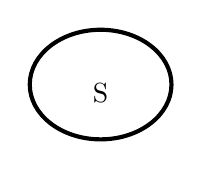
\begin{tikzpicture}
\pgftransformxscale{1.000000}
\pgftransformyscale{-1.000000}
\definecolor{dialinecolor}{rgb}{0.000000, 0.000000, 0.000000}
\pgfsetstrokecolor{dialinecolor}
\definecolor{dialinecolor}{rgb}{1.000000, 1.000000, 1.000000}
\pgfsetfillcolor{dialinecolor}
\definecolor{dialinecolor}{rgb}{1.000000, 1.000000, 1.000000}
\pgfsetfillcolor{dialinecolor}
\pgfpathellipse{\pgfpoint{7.403364\du}{8.500000\du}}{\pgfpoint{1.706967\du}{0\du}}{\pgfpoint{0\du}{1.320203\du}}
\pgfusepath{fill}
\pgfsetlinewidth{0.100000\du}
\pgfsetdash{}{0pt}
\pgfsetdash{}{0pt}
\pgfsetmiterjoin
\definecolor{dialinecolor}{rgb}{0.000000, 0.000000, 0.000000}
\pgfsetstrokecolor{dialinecolor}
\pgfpathellipse{\pgfpoint{7.403364\du}{8.500000\du}}{\pgfpoint{1.706967\du}{0\du}}{\pgfpoint{0\du}{1.320203\du}}
\pgfusepath{stroke}
% setfont left to latex
\definecolor{dialinecolor}{rgb}{0.000000, 0.000000, 0.000000}
\pgfsetstrokecolor{dialinecolor}
\node at (7.403364\du,8.695000\du){S};
\end{tikzpicture}
